\documentclass{article}
\usepackage[utf8]{inputenc}
\usepackage[
backend=biber,
sorting=ynt
]{biblatex}
\addbibresource{sstoehr.bib}
\usepackage{multirow}
\usepackage{graphicx}
\graphicspath{{./images/}}

\title{IRT Dreamscapes:

A Case Study Using First Person Image Rehearsal Therapy for Post-Traumatic Nightmares Associated with Sexual Assault}
\author{Shannon Stoehr}
\date{May 2022}

\begin{document}

\maketitle

\begin{figure}[htbp]
    \centering
    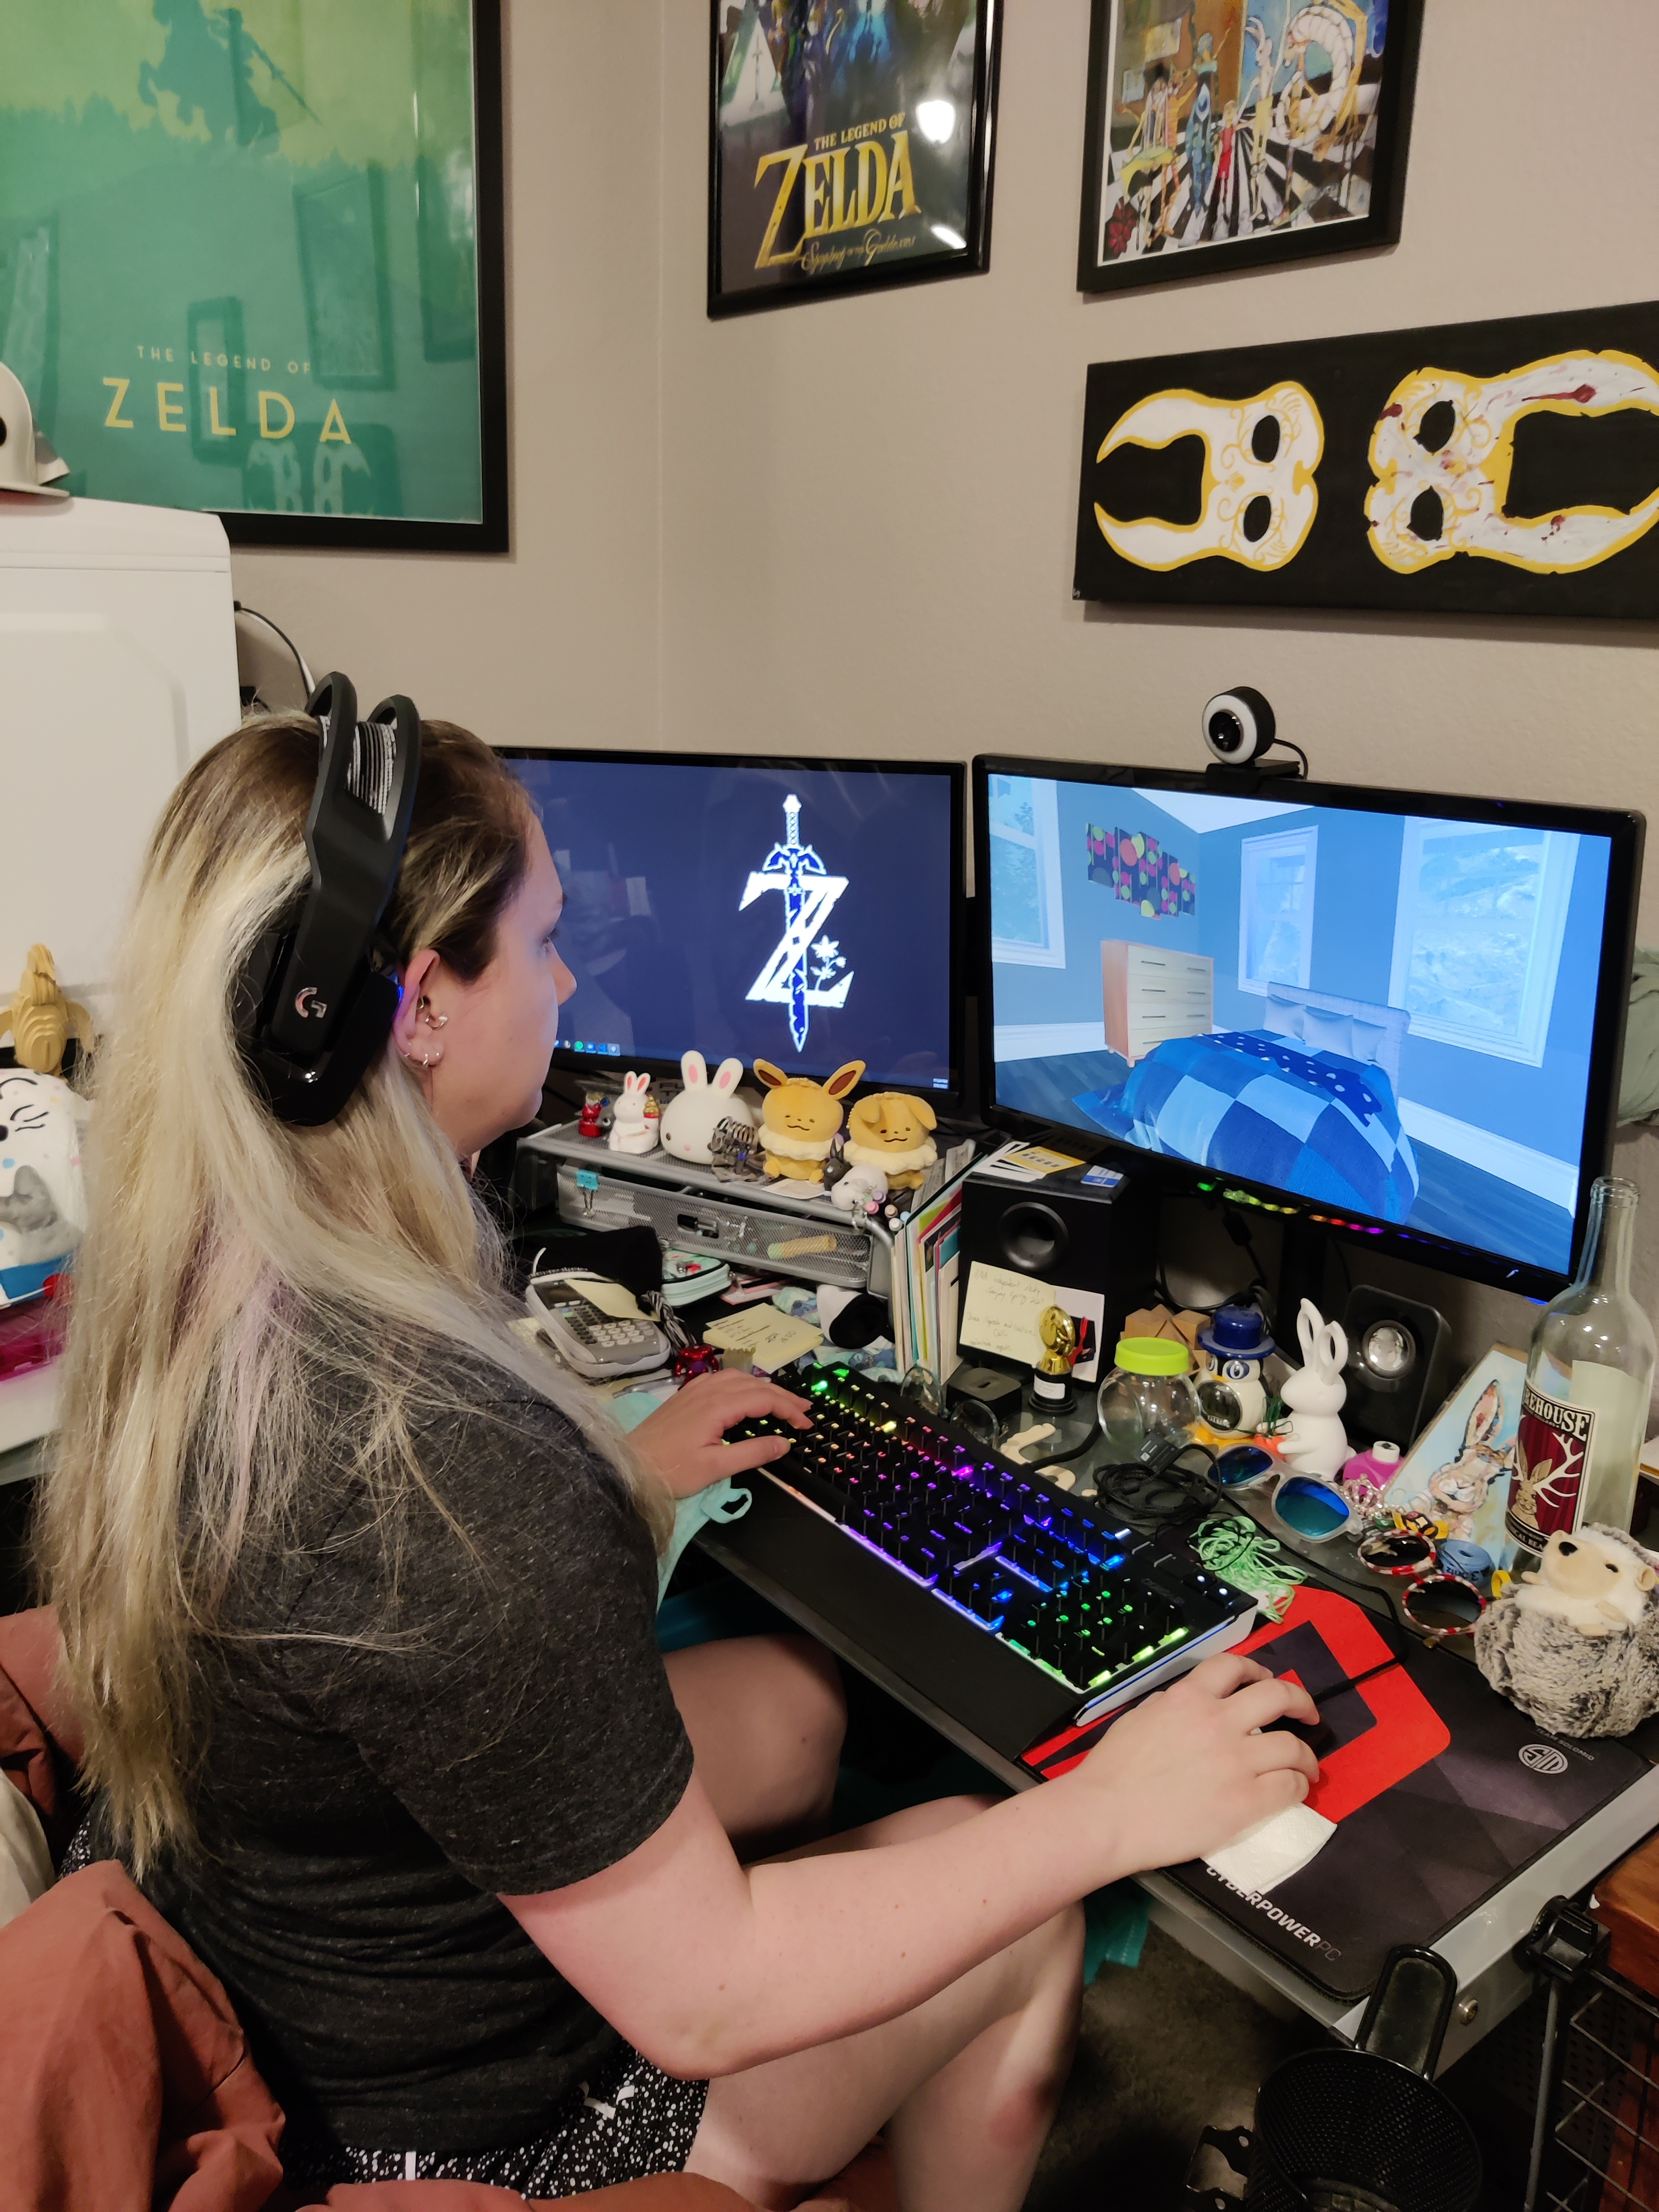
\includegraphics[width=1\textwidth]{images/irt_exp.jpg}
    \caption{Utilizing a unique dreamscape.}
\end{figure}

\section*{Abstract}

Nightmares are a common side effect of post traumatic stress disorder (PTSD), especially in sexual assault victims. Image rehearsal therapy (IRT) has been proven to be an effective treatment for nightmares in individuals with PTSD. The Disturbing Dream and Nightmare Severity Index (DDNSI) was used to assess the intensity and severity of nightmares of one female participant. She was assessed for 35 days: 20 using no IRT and 15 using the IRT Dreamscapes application. Overall her nightmare frequency, awakened frequency, nightmare intensity, and next day effects decreased, but the results were not statistically significant. These results suggest that further investigation would be worthwhile with more subjects afflicted with the same problems.

\section*{Introduction}

According to the Rape, Abuse \& Incest National Network (RAINN) an American is sexually assaulted every 68 seconds: one in six women and one in thirty three men will be sexually assaulted in their lifetimes \cite{RAINN}. A 2018 study from the World Health Organization found that nearly one in three women worldwide have been victims of sexual or physical violence and noted that this can lead to post traumatic stress disorder (PTSD) and/or other anxiety disorders, sleep difficulties, depression, and suicide attempts \cite{WHO}. PTSD can include persistent nightmares, which in turn lead to more sleep difficulties including restless sleep, insomnia, and disturbing emotions and images that are re-lived once awake \cite{KrakowZadraClinical}. Krakow and Zadra outlined the process of IRT in 2006 consisting of two components: helping patients consider their nightmares as a learned behavior and training patients about implementing specific imagery steps to reduce nightmares \cite{KrakowZadraClinical}.

As sexual assault is a disturbingly common problem for people all over the world, designing a more accessible IRT interface that utilizes computer animation would be helpful to individuals with PTSD that suffer from nightmares. Some three-dimensional applications have been developed: McNamara and colleagues developed the ReScript system that allows users to manipulate threatening images into less scary images in order to lessen anxiety and gain cognitive control over intrusive imagery \cite{McNamara}. The treatment was found to be effective, but it focused on generic threatening images (an example given was a great white shark approaching) \cite{McNamara} rather than specific, interactive scenarios from participants’ dreams.

Later on, the BRAVEMIND virtual reality system was developed by the US Army for helping combat veterans with PTSD. This allows therapists to recreate scenes of traumatic incidents for combat veterans during sessions, including an Afghan village and an Iraqi marketplace \cite{BRAVEMIND}. Originally designed in 2005, the system was updated to include more scenarios running on the Unity Game Engine in 2011 \cite{Rizzo}. Using the BRAVEMIND system in combat-related PTSD showed statistically and clinically significant improvements in patients \cite{Rizzo}. The team behind BRAVEMIND intends to update the system to include scenarios involving military sexual trauma, but this has yet to be released \cite{Rizzo}. This lack of civilian access to a helpful therapeutic tool is where the IRT Dreamscapes application comes in.

This study aims to create a more accessible and versatile system that allows civilian users to interact with their own nightmare scenarios (dreamscapes) in order to proceed with IRT. Nightmares for people that have PTSD resulting from sexual violence can vary widely: people's fears and phobias can be specific to their traumatic event (ex. specifics related to the assailant such as the car they drove) or more generalized (ex. fear of being in crowds, fear of being alone) \cite{WU}. This system needs to be able to cover a wider variety of scenarios and settings, ultimately becoming a generalized tool that anyone with any kind of nightmare can use. Generally it will not recreate the specific traumatic event itself: according to Duke et al. the events leading up to a traumatic experience are the most common type of memory intrusion in patients with PTSD \cite{Duke}, so that is where the focus will be for these custom made IRT Dreamscapes.

\section*{Methodology}
\subsection*{Participant}

The volunteer participant for this case study is a 28 year old woman formally diagnosed with PTSD in 2020 by her psychologist. This diagnosis is related to sexual assault and abuse by a previous partner.

\subsection*{Equipment}

A Windows 10 personal computer was used for this study. This computer was equipped with an Intel(R) Core(TM) i5-6600K CPU @ 3.50 GHz and a NVIDIA GeForce GTX 1060 6GB graphics card. Study materials were shown on an Acer GN246HL 144Hz monitor. The IRT Dreamscapes application was created on the Unity Game Engine using editor version 2021.3.0f1. All surveys and journals were created using Google Forms. Data analysis was completed using Google Sheets.

\subsection*{Methods}

The participant initially filled out a survey \cite{IRTIntake} to determine the appropriateness of her participation and record baseline nightmare frequency and severity. This survey was based off of the Disturbing Dream and Nightmare Severity Index (DDNSI) \cite{UPenn}. This measure has been determined to be reliable in terms of internal consistency and test-retest reliability by Lee, Krakow, and Suh in 2021 \cite{Lee}. The participant reported that on average she has nightmares four times per week and they will occasionally wake her up. These nightmares generally involve being trapped in a house with her abuser with no way out (using five words two describe her dreams she reported "trapped, abuser, alone, isolated, house"). She rates her nightmares of moderate intensity and overall considers the problem to be severe. Using the scoring guide of the DDNSI she scored a 16, which, being >10, would indicate a nightmare disorder \cite{UPenn}.

Daily journals were collected over the course of the study \cite{IRTDaily}, also based off of the DDNSI. Between April 1 and April 15 the participant was instructed to document any nightmares, including their content (five words/short phrases describing the subject(s), setting(s), or theme(s) of the nightmare) as shown in table \ref{ContentCompare}, intensity (using the DDNSI intensity scale), effect on daily activities afterwards (0 being not at all, 3 being severe incapacitation), and whether or not they woke her up before her morning alarm.

\begin{table}[htbp]
\centering
\begin{tabular}{||c c c||}
 \hline
 Content& no IRT& IRT\\
 \hline
 trapped & 91.6\% & 57.1\%\\
 house & 75\% & 66.6\% \\
 abuser & 66.6\% & 57.1\% \\
 alone & 58.3\% & 14.3\% \\
 abandoned & 25\% & 14.3\% \\
 middle of nowhere & 8.3\% & 0\% \\
 mountains & 8.3\% & 0\% \\
 swamp & 8.3\% & 0\% \\
 finals* & 0\% & 28.6\% \\
 school* & 0\% & 28.6\% \\
 presenting* & 0\% & 14.3\% \\
 \hline
\end{tabular}
\caption{A comparison of the percentage of the participant's nightmares containing specific content before using IRT and while using IRT. *this content appeared when the participant reported specific school stressors in the daily journal, which happened to be during the IRT period of the study}
\label{ContentCompare}
\end{table}

Between April 16 and April 20 the participant continued documenting nightmares in the same fashion, but she was also instructed to think about changing the dream in any way she wishes and document it \cite{IRTDailyChange}, as recommended by Krakow and Zadra \cite{KrakowZadraPP}. The first two days her response was "escape," then she added "support" on day three and "justice" on days four and five. Between April 1 and April 20 the participant had eleven nightmares and was awoken four time before her alarm.

After collecting the input from the daily journals as well as the input for the imagined changes to the typical dream, the IRT Dreamscapes application was designed to include aspects of the reported nightmares and aspects of the changed dream from both journals. A scenario was created that involved placing the participant inside of an upstairs bedroom in a two story house. The goal was to rehearse escaping from the house and the abuser and traveling to the police stationed at the back of the property lot. The environment was limited to be the house and an extended backyard. The property was surrounded by mountains to invoke a sense of isolation. An avatar representing the abuser was included on the main floor in the living room: according to Davis et al. it is necessary to engage the fear network for this type of therapy to work rather than replacing the entire nightmare with a pleasant scene \cite{Davis}. From April 21 to May 5 the participant spent ten minutes per day in the application rehearsing the changed dream, including speaking at key moments (eg. saying "I am leaving" out loud as she left the house in the application). She returned to recording in the original daily journal as well \cite{IRTDaily}. The overall results of the study are in table \ref{NightmareCompare}.

\section*{Results}

\begin{table}[htbp]
\centering
\begin{tabular}{||c c c||}
 \hline
 Metric & no IRT & IRT \\
 \hline
 Total Nightmares & 12/20 & 7/15\\
 Frequency Nightmare Nights & 0.60 & 0.466 \\
 Standard Deviation of Frequency Nightmare Nights & 0.502 & 0.516 \\
 Total Awakened Nights & 4/20 & 0/15 \\
 Frequency Awakened Nights & 0.2 & 0 \\
 Standard Deviation Frequency Awakened Nights & 0.410 & 0 \\
 Average Nightmare Intensity & 3.5 & 1.85 \\
 Standard Deviation Nightmare Intensity & 0.90 & 1.07 \\
 Average Next Day Effect & 1.33 & 0.29 \\
 Standard Deviation Next Day Effect & 0.45 & 0.41 \\
 \hline
\end{tabular}
\caption{A comparison of the total number of nightmares, frequency of nights with nightmares, standard deviation of frequency of nights with nightmares, total number of nights awakened, frequency of nights awakened, standard deviation of frequency of nights awakened, average intensity of the nightmare, standard deviation of average intensity of the nightmare, the average next day effect of the nightmare, and the standard deviation of the average next day effect of the nightmare before using IRT and while using IRT.}
\label{NightmareCompare}
\end{table}

\begin{figure}[htbp]
    \centering
    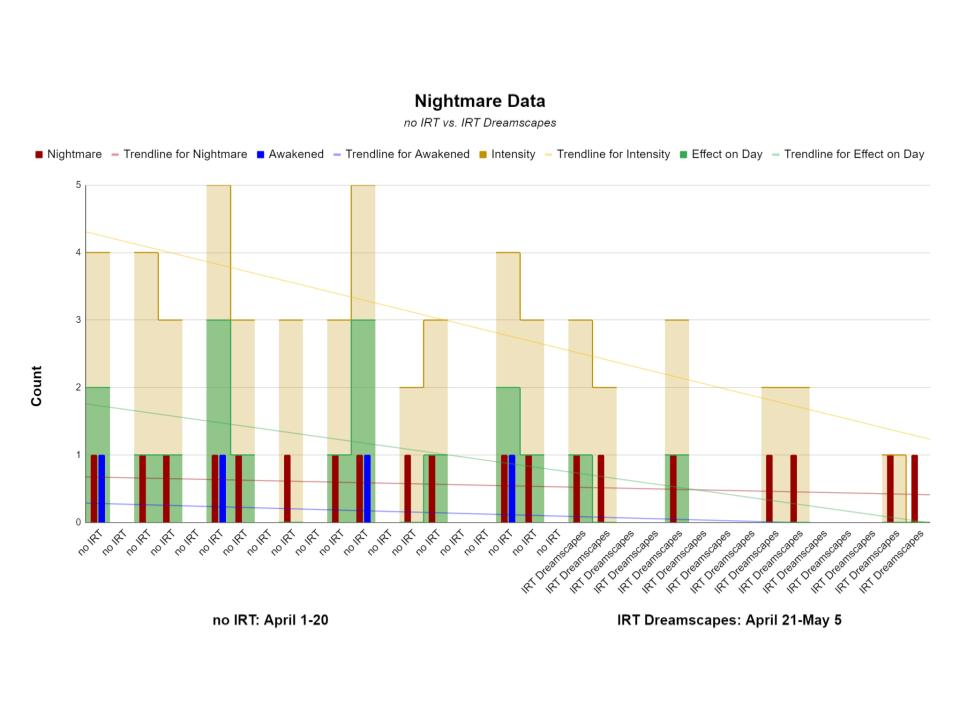
\includegraphics[width=1\textwidth]{images/nightmare_data.jpg}
    \caption{The results of the study.}
    \label{fig:nightmaredata}
\end{figure}

Overall, there was a decrease in the frequency of nightmare nights, frequency of awakened nights, average nightmare intensity, and average next day effects when IRT Dreamscapes was used, as seen in figure \ref{fig:nightmaredata}.

The non-IRT data was compared to the IRT data using a one-tailed, two-sample unequal variance T-Test in Google Sheets, as shown in table \ref{NightmareStats}.

\begin{table}[htbp]
\centering
\begin{tabular}{||c c c c||}
 \hline
 Metric & Degrees of Freedom & t-Test & t(0.95) \\
 \hline
 Frequency Nightmare Nights & 2 & 0.22526 & 2.920 \\
 Frequency Awakened Nights & 2 & 0.02104 & 2.920 \\
 Average Nightmare Intensity & 7 & 0.00288 & 1.895 \\
 Average Next Day Effect & 4 & 0.00335 & 2.132 \\
 \hline
\end{tabular}
\caption{The one-tailed, two-sample unequal variance t-Test results for each metric, comparing non-IRT and IRT data.}
\label{NightmareStats}
\end{table}

\begin{figure}[htbp]
    \centering
    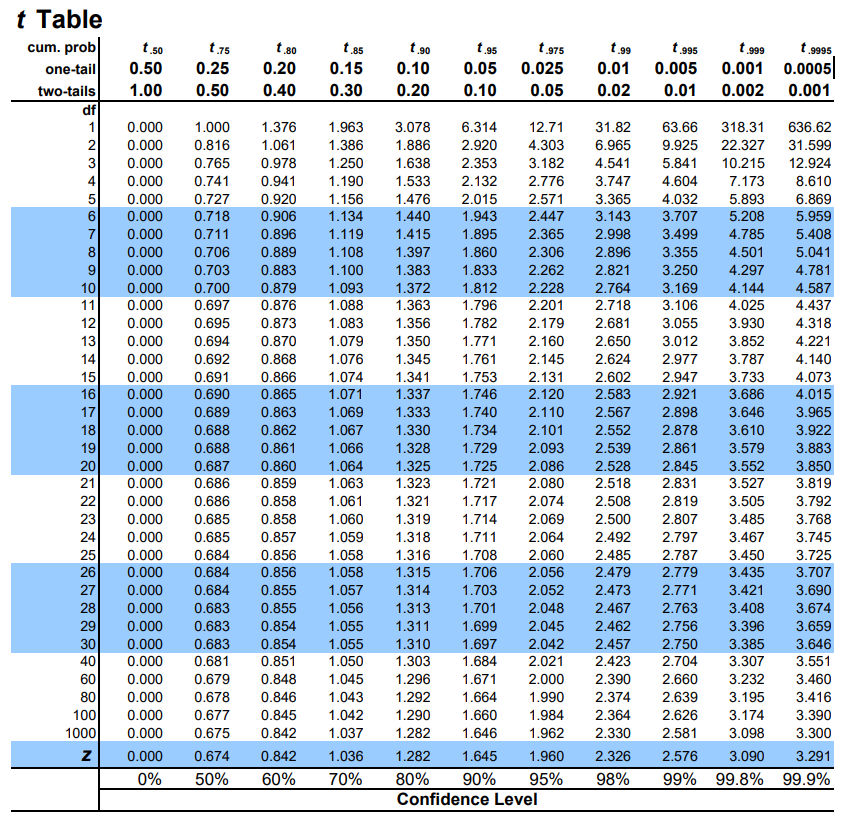
\includegraphics[width=1\textwidth]{images/t-table.jpg}
    \caption{The T Distribution Critical Values Table from Grade Calculator.}
    \label{fig:ttable}
\end{figure}

Comparing this data to the T Distribution Critical Values Table \cite{TTable} in figure \ref{fig:ttable}, none of the t-Test results show statistical significance for any of the metrics, as they were all less than the t(0.95) values for their respective degrees of freedom.

\section*{Discussion}

IRT has been proven to be an effective tool in treating PTSD symptoms, nightmare frequency, and sleep quality, and the positive effects will last 6-12 months after treatment \cite{Casement}. This is an important treatment option for individuals that may be resistant or averse to medication treatments or exposure therapies \cite{KrakowJAMA}. Combined treatment of IRT and cognitive behavioral therapy can improve sleep quality better than IRT alone, but the combined therapies will not improve PTSD symptoms or nightmares \cite{Casement}. Having an accessible IRT option is crucial to civilian PTSD patients. Further research should focus on developing more intricate IRT systems that allow users to customize their dreamscapes on their own instead of relying on a designer to create an approximated dreamscape to be used. When IRT Dreamscapes has more customization options available then it will become a tool that is more accessible to a wider variety of people. Krakow believes that "the process of changing the dream is a very integral component of the program" \cite{KrakowTS}, and making the IRT Dreamscapes application more flexible will allow more people to utilize this type of therapy.

This study was limited in that there was one subject and it was conducted over the course of only 35 days (20 with no IRT, 15 with IRT). It would be worthwhile repeating this study over a longer period of time with more subjects and a more robust IRT Dreamscapes application.

\section*{Acknowledgements}

I wish to thank Unity for having such wonderful tutorials and assets to work with. I would also like to thank my husband who supported me throughout this entire study.

\printbibliography[
heading=bibintoc,
title={References}
]

\end{document}